%!TEX root = ../template.tex
%%%%%%%%%%%%%%%%%%%%%%%%%%%%%%%%%%%%%%%%%%%%%%%%%%%%%%%%%%%%%%%%%%%%
%% appendix-benchmarks.tex
%% Complete benchmark results summarised in Chapter 6 (Evaluation)
%% The tables and charts are placed in sequence rather than as floats; each chart sits below its
%% table at the full text width. \raggedbottom keeps the space a block leaves at the foot of a page
%% there instead of spreading it between the blocks.
%%%%%%%%%%%%%%%%%%%%%%%%%%%%%%%%%%%%%%%%%%%%%%%%%%%%%%%%%%%%%%%%%%%%
\chapter{Benchmark Results}
\label{app:benchmarks}
\raggedbottom

This appendix gives the complete results of the experiments summarised in
Table~\ref{tab:eval-summary} (Section~\ref{sec:eval-resolution}), measured as described in
Section~\ref{sec:eval-methodology}. All times are in microseconds per operation. Table~\ref{tab:eval-notation}
lists the symbols. Internal calls are distributed round-robin over the $F$ distinct functions, and
unless stated otherwise the registry always hits ($R{=}F$). Two points have a 99.9\% confidence
interval close to their own value and should be read as noise: T9 at $K{=}10$, $R_0{=}10$
($874 \pm 732\,\mu$s), and T13 at depth~2 ($69.0 \pm 40.8\,\mu$s).

\noindent\begin{minipage}{\textwidth}
  \centering
  \captionof{table}{Notation used throughout the evaluation.}
  \label{tab:eval-notation}
  \begin{tabular}{|c|>{\raggedright\arraybackslash}p{0.8\textwidth}|}
    \hline
    \textbf{Symbol} & \textbf{Meaning} \\
    \hline
    $N$ & total number of \texttt{call} steps in the workflow (internal or external), $N = I + E$ \\
    \hline
    $I$ & number of internal calls (repetitions counted) \\
    \hline
    $E$ & number of external calls (repetitions counted) \\
    \hline
    $R$ & number of entries in the registry file when it is read/written \\
    \hline
    $F$ & number of \emph{distinct} internal functions the workflow references \\
    \hline
    $K$ & number of successive registry writes (T8, T9) \\
    \hline
    $R_0$ & number of entries in the registry before the writes (T8, T9) \\
    \hline
  \end{tabular}
\end{minipage}

\FloatBlock
\section{Resolution Against the Reference Resolver (T2--T5)}

T2 re-reads the registry on every internal call (naive path): each read costs about $10.3\,\mu$s
plus $0.17\,\mu$s per entry, so up to $R \approx 60$ the fixed cost of opening and parsing the file
dominates. T3 compares that path with the single read by calling the store's lookup $N$ times,
without building a workflow (Table~\ref{tab:eval-t3}); T4 and T5 do the same on a real
\texttt{Workflow} object.

\bigskip
\noindent\begin{minipage}{\textwidth}
  \centering
  {\captionsetup{textfont=sf}\captionof{table}{T2: per-call resolution cost as a function of registry size $R$, with the registry
  re-read on every internal call: total time divided by $N$, averaged over $N \in \{1, 10, 50,
  200\}$.}
  \label{tab:eval-t2}}
    \small
    \begin{tabular}{|r|r|}
      \hline
      \textbf{$R$} & \textbf{Per call ($\mu$s)} \\
      \hline
      1    & 10.5  \\
      \hline
      10   & 11.9  \\
      \hline
      50   & 18.3  \\
      \hline
      200  & 44.5  \\
      \hline
      1000 & 183.4 \\
      \hline
    \end{tabular}
  \normalsize

  \medskip
  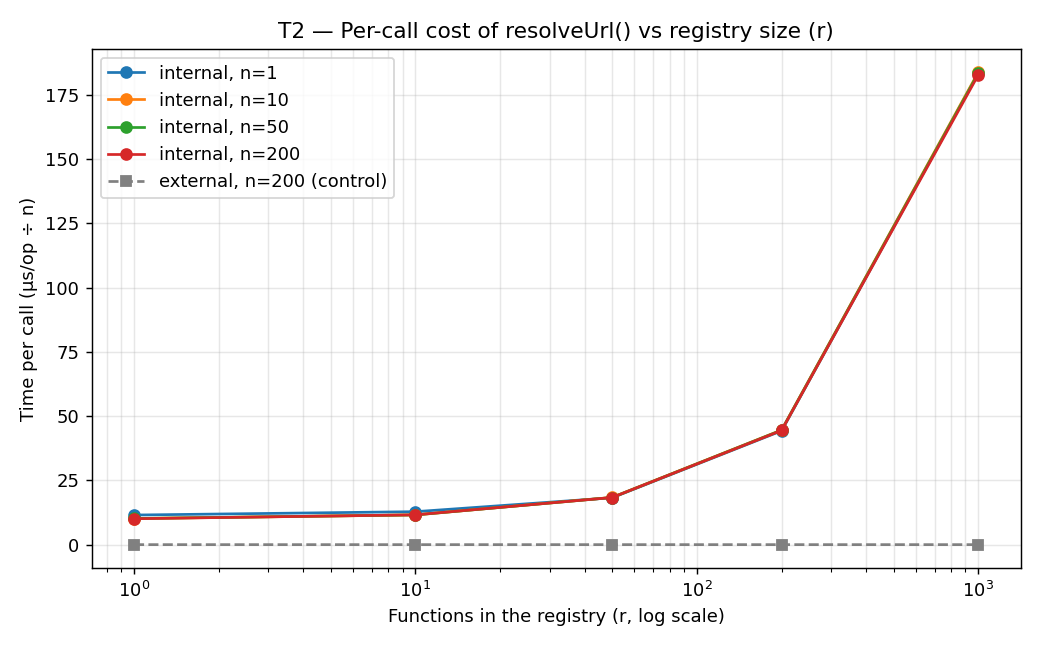
\includegraphics[width=\textwidth,height=0.45\textheight,keepaspectratio]{images/benchmarks/T2_registry_scaling.png}
  {\captionof{figure}{T2: per-call resolution cost as a function of registry size $R$, for $N \in \{1, 10,
  50, 200\}$ internal calls. The external-call control does not read the registry.}
  \label{fig:eval-t2}}
\end{minipage}

\bigskip
\noindent\begin{minipage}{\textwidth}
  \centering
  {\captionsetup{textfont=sf}\captionof{table}{T3: total resolution time ($\mu$s), naive (per-call read) vs.\ optimised (single
  read).}
  \label{tab:eval-t3}}
  \small
  \begin{tabular}{|l|r|r|r|r|}
    \hline
     & $N{=}1$ & $N{=}10$ & $N{=}50$ & $N{=}200$ \\
     \hline
    naive, $R{=}1$        & 9.8  & 98.0     & 492      & 1\,999    \\
    \hline
    optimised, $R{=}1$    & 10.0 & 10.0     & 10.1     & 10.3      \\
    \hline
    naive, $R{=}50$       & 17.9 & 180      & 901      & 3\,630    \\
    \hline
    optimised, $R{=}50$   & 18.4 & 18.3     & 18.5     & 18.5      \\
    \hline
    naive, $R{=}1000$     & 183  & 1\,839   & 9\,239   & 36\,670   \\
    \hline
    optimised, $R{=}1000$ & 182  & 183      & 182      & 184       \\
    \hline
  \end{tabular}
\end{minipage}

\bigskip
\noindent\begin{minipage}{\textwidth}
  \centering
  \begin{minipage}[t]{0.48\textwidth}
    \centering
    {\captionsetup{textfont=sf}\captionof{table}{T4: naive resolution time ($\mu$s) of a real workflow, $F$ distinct functions vs.\
    $N$ calls, $R{=}F$.}
    \label{tab:eval-t4-naive}}
    \small
    \begin{tabular}{|r|r|r|r|r|r|}
      \hline
      $F\backslash N$ & 1 & 5 & 10 & 50 & 200 \\
      \hline
      1  & 10.4 & 52.3 & 105 & 525 & 2\,069 \\
      \hline
      2  & 10.8 & 53.0 & 106 & 534 & 2\,142 \\
      \hline
      5  & 11.1 & 53.9 & 108 & 543 & 2\,150 \\
      \hline
      10 & 11.6 & 58.5 & 116 & 582 & 2\,333 \\
      \hline
      20 & 13.3 & 66.6 & 133 & 665 & 2\,650 \\
      \hline
      50 & 18.7 & 92.5 & 185 & 929 & 3\,694 \\
      \hline
    \end{tabular}
  \end{minipage}\hfill
  \begin{minipage}[t]{0.48\textwidth}
    \centering
    {\captionsetup{textfont=sf}\captionof{table}{T4: optimised (single-read) resolution time ($\mu$s) of a real workflow, same grid
    as Table~\ref{tab:eval-t4-naive}.}
    \label{tab:eval-t4-optimized}}
    \small
    \begin{tabular}{|r|r|r|r|r|r|}
      \hline
      $F\backslash N$ & 1 & 5 & 10 & 50 & 200 \\
      \hline
      1  & 10.2 & 11.1 & 12.2 & 20.7 & 54.7 \\
      \hline
      2  & 10.4 & 11.2 & 12.2 & 21.1 & 54.1 \\
      \hline
      5  & 10.7 & 11.6 & 12.7 & 21.5 & 54.1 \\
      \hline
      10 & 11.5 & 12.7 & 13.8 & 22.5 & 55.8 \\
      \hline
      20 & 13.4 & 14.2 & 15.2 & 24.0 & 57.9 \\
      \hline
      50 & 18.5 & 19.4 & 20.8 & 29.4 & 63.3 \\
      \hline
    \end{tabular}
  \end{minipage}
\end{minipage}

\bigskip
\noindent\begin{minipage}{\textwidth}
  \centering
  {\captionsetup{textfont=sf}\captionof{table}{T5: resolution time ($\mu$s) vs.\ registry size $R$, $F{=}10$/$N{=}50$ fixed.}
  \label{tab:eval-t5}}
    \small
    \setlength{\tabcolsep}{4pt}
    \begin{tabular}{|r|r|r|r|}
      \hline
      \textbf{$R$} & \textbf{naive} & \textbf{opt.} & \textbf{speedup} \\
      \hline
      10   & 589     & 22.6 & 26.1 \\
      \hline
      20   & 666     & 23.9 & 27.9 \\
      \hline
      50   & 930     & 29.3 & 31.8 \\
      \hline
      100  & 1\,378  & 37.8 & 36.5 \\
      \hline
      200  & 2\,246  & 54.9 & 40.9 \\
      \hline
      1000 & 9\,487  & 205  & 46.3 \\
      \hline
    \end{tabular}
  \normalsize

  \medskip
  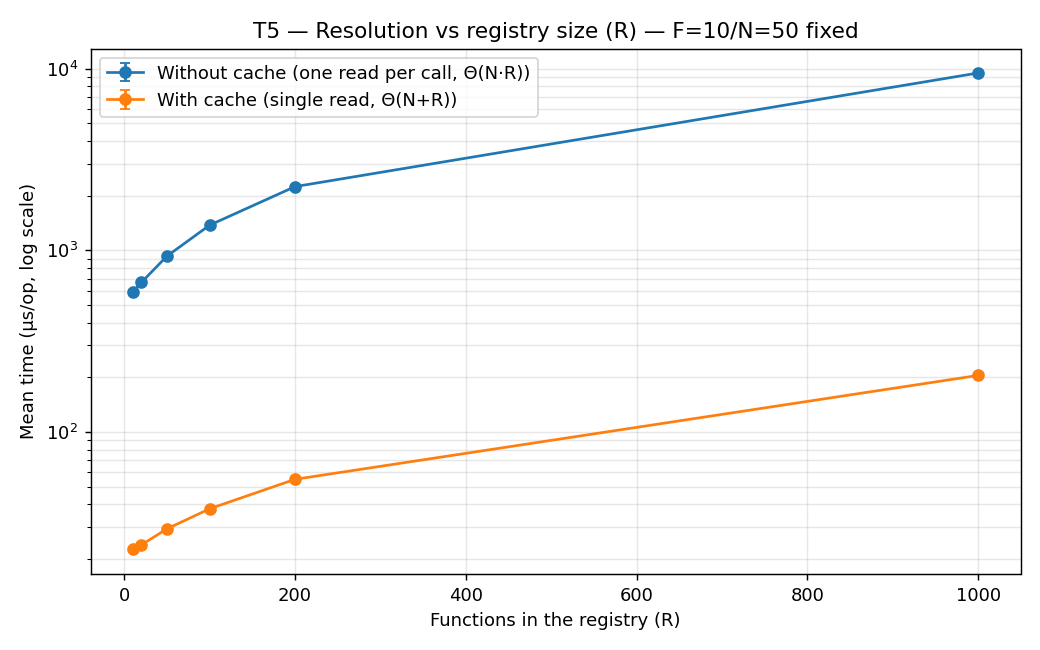
\includegraphics[width=\textwidth,height=0.45\textheight,keepaspectratio]{images/benchmarks/T5_resolution_by_registry.png}
  {\captionof{figure}{T5: resolution time against registry size $R$ with $F{=}10$/$N{=}50$ fixed,
  per-call read against single read (logarithmic vertical axis). Both paths grow with $R$, and the
  gap between them widens with it.}
  \label{fig:eval-t5}}
\end{minipage}

\FloatBlock
\section{Production Resolvers (T6, T7)}

\bigskip
\noindent\begin{minipage}{\textwidth}
  \centering
  \begin{minipage}[b]{0.48\textwidth}
    \centering
    {\captionsetup{textfont=sf}\captionof{table}{T6: AWS provider: resolution time ($\mu$s) of the real resolver
    (\texttt{Aws\allowbreak Internal\allowbreak Function\allowbreak Resolver}), $R{=}F$, with the
    single-read optimisation.}
    \label{tab:eval-t6}}
    \small
    \begin{tabular}{|l|r|r|r|r|r|}
      \hline
      $F\backslash N$ & 1 & 5 & 10 & 50 & 200 \\
      \hline
      1  & 9.9  & 10.3 & 10.9 & 13.8 & 24.6 \\
      \hline
      2  & 10.2 & 11.0 & 11.4 & 14.7 & 26.3 \\
      \hline
      5  & 11.0 & 11.2 & 11.7 & 15.3 & 27.6 \\
      \hline
      10 & 11.7 & 12.2 & 12.7 & 16.3 & 29.1 \\
      \hline
      20 & 14.4 & 14.8 & 14.4 & 19.7 & 34.5 \\
      \hline
      50 & 20.0 & 20.3 & 20.3 & 26.6 & 47.5 \\
      \hline
    \end{tabular}
  \end{minipage}\hfill
  \begin{minipage}[b]{0.48\textwidth}
    \centering
    {\captionsetup{textfont=sf}\captionof{table}{T7: GCP provider: resolution time ($\mu$s) of the real resolver
    (\texttt{Workflow\allowbreak Internal\allowbreak Function\allowbreak Resolver}), $R{=}F$, with
    the single-read optimisation and with every hit validated
    through a Cloud Run client answered locally.}
    \label{tab:eval-t7}}
    \small
    \begin{tabular}{|l|r|r|r|r|r|}
      \hline
      $F\backslash N$ & 1 & 5 & 10 & 50 & 200 \\
      \hline
      1  & 11.8 & 15.8 & 21.3 & 59.3 & 207.1 \\
      \hline
      2  & 12.1 & 16.4 & 21.3 & 61.3 & 209.1 \\
      \hline
      5  & 13.0 & 17.5 & 21.9 & 62.4 & 211.5 \\
      \hline
      10 & 15.1 & 18.4 & 23.1 & 60.2 & 199.1 \\
      \hline
      20 & 15.4 & 19.2 & 24.0 & 61.5 & 205.9 \\
      \hline
      50 & 21.9 & 25.6 & 30.6 & 67.5 & 209.0 \\
      \hline
    \end{tabular}
  \end{minipage}
\end{minipage}

\FloatBlock
\section{Registry Write Path (T8, T9)}

\bigskip
\noindent\begin{minipage}{\textwidth}
  \centering
  \begin{minipage}[b]{0.48\textwidth}
    \centering
    {\captionsetup{textfont=sf}\captionof{table}{T8: total write time ($\mu$s): $K$ successive \texttt{put} calls, initial registry
    size $R_0$.}
    \label{tab:eval-t8}}
    \footnotesize
    \setlength{\tabcolsep}{3pt}
    \begin{tabular}{|l|r|r|r|r|r|}
      \hline
      $K\backslash R_0$ & 0 & 10 & 50 & 200 & 1000 \\
      \hline
      1   & 45.5     & 48.2     & 63.8     & 114       & 490       \\
      \hline
      5   & 224      & 242      & 329      & 529       & 1\,945    \\
      \hline
      10  & 463      & 496      & 640      & 1\,041    & 3\,751    \\
      \hline
      50  & 2\,517   & 2\,706   & 3\,650   & 5\,363    & 17\,942   \\
      \hline
      100 & 5\,914   & 6\,693   & 7\,594   & 11\,515   & 36\,195   \\
      \hline
    \end{tabular}
  \end{minipage}\hfill
  \begin{minipage}[b]{0.48\textwidth}
    \centering
    {\captionsetup{textfont=sf}\captionof{table}{T9: total write time ($\mu$s): $K$ successive miss+\texttt{put} pairs, initial
    registry size $R_0$.}
    \label{tab:eval-t9}}
    \footnotesize
    \setlength{\tabcolsep}{3pt}
    \begin{tabular}{|l|r|r|r|r|r|}
      \hline
      $K\backslash R_0$ & 0 & 10 & 50 & 200 & 1000 \\
      \hline
      1   & 57.2     & 62.7     & 90.2     & 164       & 686       \\
      \hline
      5   & 298      & 323      & 427      & 769       & 2\,901    \\
      \hline
      10  & 597      & 874      & 973      & 1\,557    & 5\,751    \\
      \hline
      50  & 3\,265   & 3\,510   & 5\,051   & 8\,144    & 28\,694   \\
      \hline
      100 & 8\,369   & 8\,307   & 10\,516  & 17\,689   & 58\,572   \\
      \hline
    \end{tabular}
  \end{minipage}
\end{minipage}

\FloatBlock
\section{Match Strategy and Workflow Shape (T10--T14)}

T12 (registry size with $I{=}40$ internal calls among mixed calls) and T13 (nesting depth) have
no table: T12 goes from $20\,\mu$s at $R{=}10$ to $199\,\mu$s at $R{=}1000$, and T13 stays at
$15.8$--$19.2\,\mu$s across depths 0--5 with 20 internal calls.

\bigskip
\noindent\begin{minipage}{\textwidth}
  \centering
  {\captionsetup{textfont=sf}\captionof{table}{T10: exact vs.\ suffix match ($\mu$s), $F{=}10$/$N{=}50$ fixed.}
  \label{tab:eval-t10}}
    \small
    \begin{tabular}{|r|r|r|r|}
      \hline
      \textbf{$R$} & \textbf{exact} & \textbf{suffix} & \textbf{ratio} \\
      \hline
      10   & 22.5 & 28.8 & 1.28 \\
      \hline
      20   & 24.2 & 32.6 & 1.35 \\
      \hline
      50   & 29.2 & 40.2 & 1.38 \\
      \hline
      100  & 38.2 & 58.9 & 1.54 \\
      \hline
      200  & 55.0 & 92.6 & 1.68 \\
      \hline
      1000 & 201  & 391  & 1.95 \\
      \hline
    \end{tabular}
  \normalsize

  \medskip
  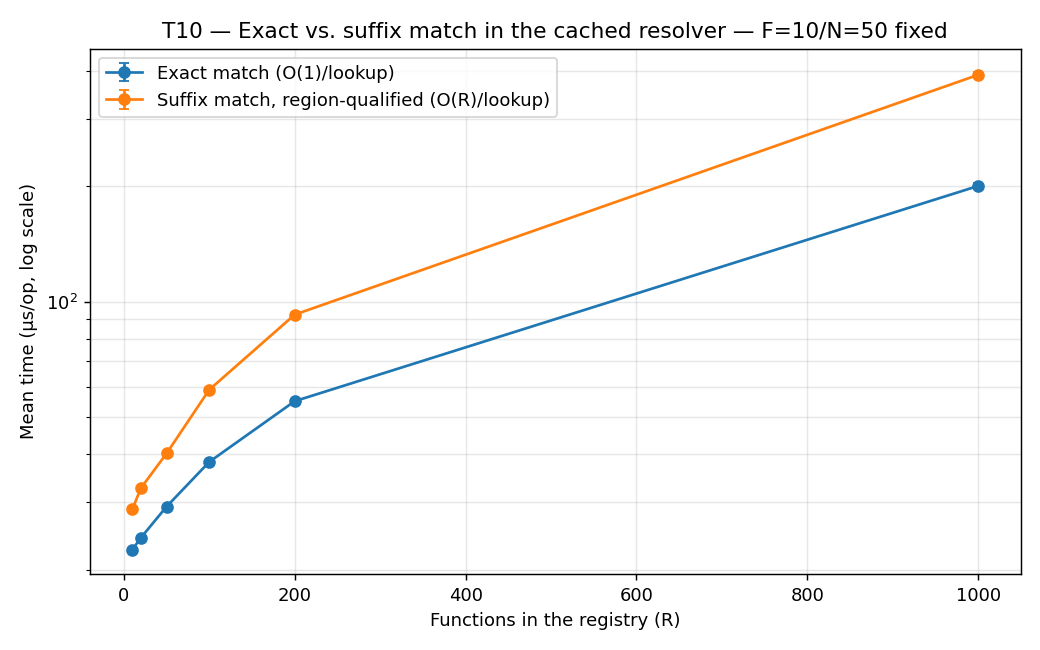
\includegraphics[width=\textwidth,height=0.45\textheight,keepaspectratio]{images/benchmarks/T10_resolution_key_match_strategy.png}
  {\captionof{figure}{T10: exact against suffix match in the single-read resolver, $F{=}10$/$N{=}50$
  fixed (logarithmic vertical axis). Both grow with $R$ because of the read, and the suffix path adds
  a scan of the loaded map on top of it.}
  \label{fig:eval-t10}}
\end{minipage}

\bigskip
\noindent\begin{minipage}{\textwidth}
  \centering
  {\captionsetup{textfont=sf}\captionof{table}{T11: resolution time ($\mu$s) of a mixed workflow with $I$ internal and
$E$ external calls, $R{=}F{=}10$ fixed.}
  \label{tab:eval-t11}}
  \small
  \begin{tabular}{|r|r|r|r|r|r|r|}
    \hline
    $I\backslash E$ & 0 & 1 & 5 & 10 & 50 & 200 \\
    \hline
    0   & 11.3 & 11.3 & 11.5 & 11.5 & 13.9 & 12.7 \\
    \hline
    1   & 11.5 & 11.7 & 11.8 & 11.8 & 14.4 & 12.7 \\
    \hline
    5   & 12.8 & 12.6 & 12.6 & 12.7 & 12.9 & 13.7 \\
    \hline
    10  & 13.7 & 13.8 & 13.8 & 13.8 & 14.0 & 14.7 \\
    \hline
    50  & 22.4 & 22.4 & 22.7 & 26.3 & 22.8 & 23.2 \\
    \hline
    200 & 55.8 & 55.9 & 56.2 & 67.1 & 57.4 & 56.8 \\
    \hline
  \end{tabular}
\end{minipage}

\bigskip
\noindent\begin{minipage}{\textwidth}
  \centering
  {\captionsetup{textfont=sf}\captionof{table}{T14: resolution time ($\mu$s) vs.\ \texttt{Parallel} branch width,
  $N = 5\times$ width, $R{=}F{=}10$.}
  \label{tab:eval-t14}}
    \small
    \begin{tabular}{|r|r|r|}
      \hline
      \textbf{Branches} & \textbf{$N$} & \textbf{Time ($\mu$s)} \\
      \hline
      1   & 5   & 12.5 \\
      \hline
      2   & 10  & 13.7 \\
      \hline
      5   & 25  & 17.0 \\
      \hline
      10  & 50  & 22.4 \\
      \hline
      20  & 100 & 33.2 \\
      \hline
      50  & 250 & 65.2 \\
      \hline
      100 & 500 & 119  \\
      \hline
    \end{tabular}
  \normalsize

  \medskip
  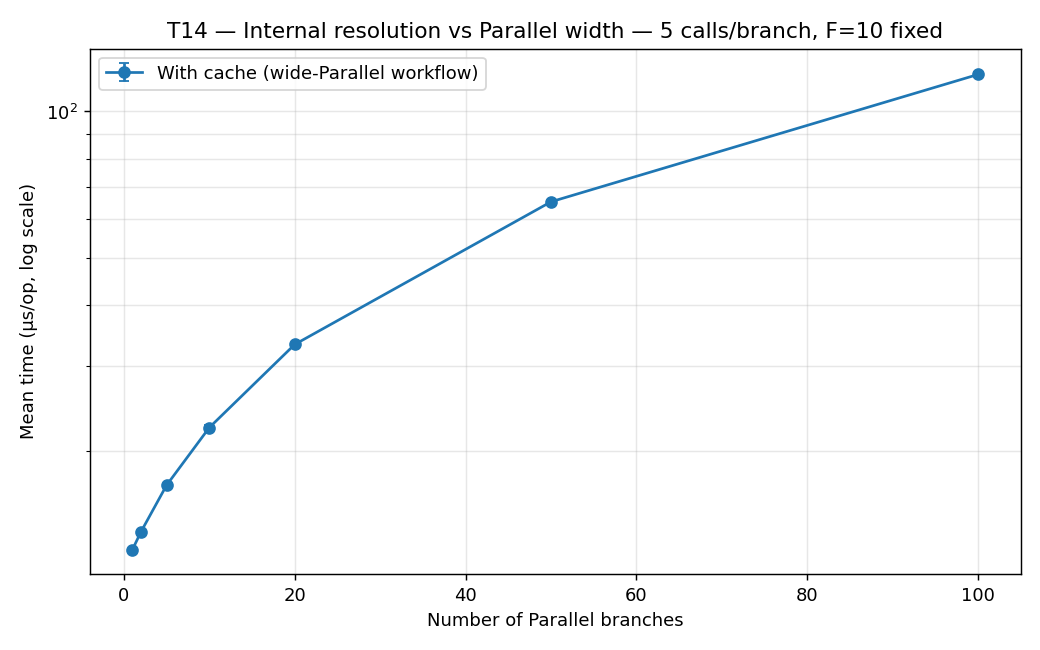
\includegraphics[width=\textwidth,height=0.45\textheight,keepaspectratio]{images/benchmarks/T14_internal_resolution_by_branch_width.png}
  {\captionof{figure}{T14: resolution time against \texttt{Parallel} branch width, five internal calls per
  branch and $R{=}F{=}10$ fixed (logarithmic vertical axis). The time follows the total number of
  leaf calls $N = 5\times\text{width}$, not the shape of the tree.}
  \label{fig:eval-t14}}
\end{minipage}
